\chapter{Deep reinforcement learning for learning high level policies}

\label{chap:deep}

In this Chapter, we describe a second way of including simulation information in hardware experiments. Instead of building feature transforms in simulation, and learning controllers on hardware, we learn robust policies in simulation and implement them on hardware. We present our experiments on the effect of policy structure on rate of transfer between simulation and hardware.

\section{Neural network policies on the ATRIAS biped}

One way of transferring information between simulation and hardware is to directly learn a robust policy in simulation and deploy it on hardware. We train a deep neural network policy for controlling ATRIAS in simulation with ground height disturbance and test it on hardware. We experiment with different neural network controller structures, and study their effect on transfer from simulation to hardware, without any domain randomization. We show that structured neural network controllers have a fast training rate in simulation as well as higher rate of transfer to hardware. The structure also gives the user the power to modify the controller, if required, without having to re-train the neural network from scratch.

Deep reinforcement learning from scratch proved to be very challenging for a high-fidelity simulation of a bipedal robot. Deep RL methods depend on randomly exploring the space to get a notion of gradient of the cost. However, for underactuated bipedal robots most regions of space have very low reward, and hence no clear gradient. Stable walking regions in the controller space can be very narrow, making it unlikely to reach a promising controller by merely random sampling. To overcome this, we used behavior cloning to initialize our actor policy using the expert feedback-based reactive controller described in Section \ref{sec:raibert_cont}. Behavior cloning learns a policy over state-action pairs from expert trajectory by finding the policy parameters $\theta$ that solve the following maximum-likelihood optimization problem, as described in  \cite{rajeswaran2017learning}: 
\begin{equation}
    maximize_\theta \sum_{(s,a^*) \in \rho_D} ln \, \pi_\theta (a^*|s)
\end{equation}
where $\rho_D$ indicates the expert's trajectory distribution, with  $a^*$ is actions that expert took, and $s$ are the states visited.

Similarly, rewards accumulated during the expert's demonstrations can be used to pre-train a Q-function by minimizing TD error \citep{sendonaris2017learning}. As the Q-function provides the guidance for policy update, a well pre-trained Q-function benefits actor training as well. 

In practice, imitation learning does not guarantee that the cloned policy can work as well as the expert due to compounding error caused by distributional shift in states seen during training and testing, as described in  \cite{ross2010efficient}. Moreover, the expert controller might not perform sufficiently well in settings where it is difficult to design a controller. For example, while our expert controller is very stable on flat ground walking, rough ground seems to present a challenge. This means that the learned policy actually has to be updated to perform well in this situation, even in simulation. Nevertheless, the expert is a good initialization for the policy and makes the learning process much faster, by overcoming the need to randomly sample. We discuss two different types of neural network controllers that can be trained to obtain a better and more robust policy. 

\subsection{Neural Network Policy}
\label{NN_P}

In our first setting, we create a general neural network policy without a lot of structure. Similar to the expert controller, we design the action space of the neural network to be horizontal and vertical ground  reaction forces (GRFs) $F_z$, $F_x$ and the swing leg foot place location $x_p$. The input space is the state of the CoM:  (x,$v_{act}$,$z$,$\dot{z}$,$\theta$,$\dot{\theta}$). This means that the structure of the neural network policy becomes:
\begin{equation}
    \pi(x,v_{act},z,\dot{z},\theta,\dot{\theta})_{NN} \rightarrow  (F_z, F_x,x_p)
\end{equation}
The stance and swing control pipeline is similar to the expert and shown in Figure \ref{fig:NN_process}. The expert controller described in Section \ref{sec:raibert_cont} is used to pre-train the neural network policy to walk on flat ground.

\begin{figure}[!h]
	\centering
	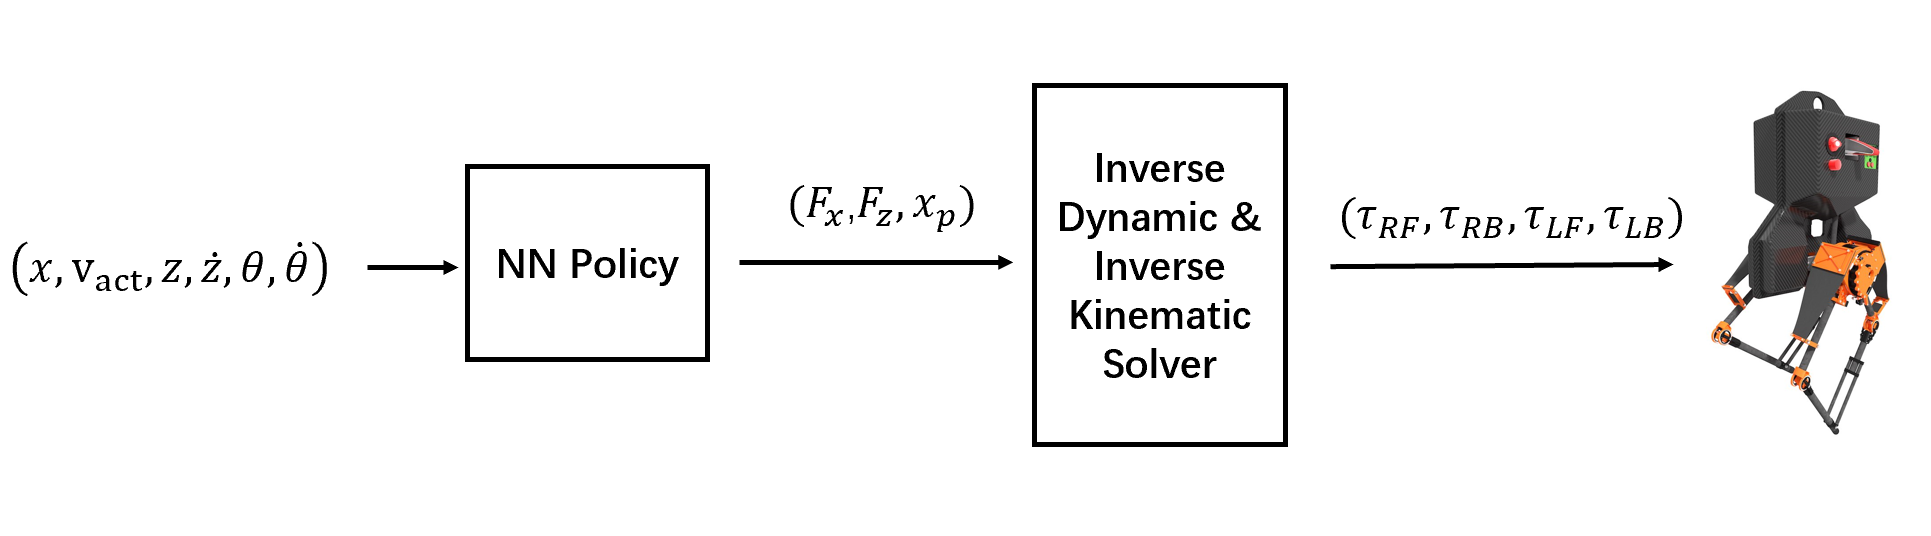
\includegraphics[width=.7\textwidth]{./img/NN.PNG}
    \caption{Pipeline of our first neural network policy for controlling ATRIAS. Here $\tau_{RF},\tau_{RB},\tau_{LF},\tau_{LB}$ are torques in the right leg's front and back and left leg's front and back motors.}
    \label{fig:NN_process}
\end{figure}

While this policy still has the information about dynamics constraints of the robot through the inverse dynamics and inverse kinematics blocks, it loses the well-defined structure of the expert. This means that the output of the neural network is unpredictable, and the user does not have a lot of control over the behavior of the robot. Roboticists typically prefer controllers that can be understood and predictable, as well as can be modified if needed. In our second controller, we try to emulate this shared autonomy, which lets the user control the overall behavior of the robot, and the neural network helps improve the user-designed policy through deep reinforcement learning.

\subsection{Neural Network in the Heuristic Policy}\label{NN_HP}

In our second setting, instead of directly predicting the vertical and horizontal ground reaction force $ (F_z, F_x,x_p)$ as well as desired swing leg foot place location $x_p$, we use a neural network as part of the feedback based reactive stepping policy, described in Section \ref{sec:raibert_cont}. 
While the original policy has a fixed desired torso lean $\theta_{des}$, desired CoM height $z_{des}$ and fixed structure for $x_p$, we learn these as a function of the state of the CoM using a neural network. The neural network now takes the state of the CoM as input, and predicts the desired torso pitch, CoM height and an offset on the footstep location.
\begin{align}
  \pi(x,v_{act},z,\dot{z},\theta,\dot{\theta})_{HP} \rightarrow  (\theta_{NN}, z_{NN},x_{NN}) 
\end{align}

When inserted into the expert controller, this gives a structured neural network policy, where neural network outputs are used as part of a heuristic policy. It is worth noting that this policy is capable of generating the same outputs as the general neural network policy. For example, for any desired $F_{x}$ profile, it is always possible to find a $\theta_{NN}$ given $K_{pt}$, $K_{dt}$, $\theta$ and $\dot{\theta}$. The pipeline is illustrated in Figure \ref{fig:H_process}.

\begin{align}
F_x = K_{pt}(\theta_{NN} - \theta) + K_{dt}(-\dot{\theta}) \\
F_z = K_{pz}(z_{NN}-z) + K_{dz}( - \dot{z}) \\
x_p=k(v_{act}-v_{tgt}) + 0.5 \cdot v \cdot T + x_{NN}\label{x_p eq}
\end{align}


\begin{figure}[!h]
	\centering
	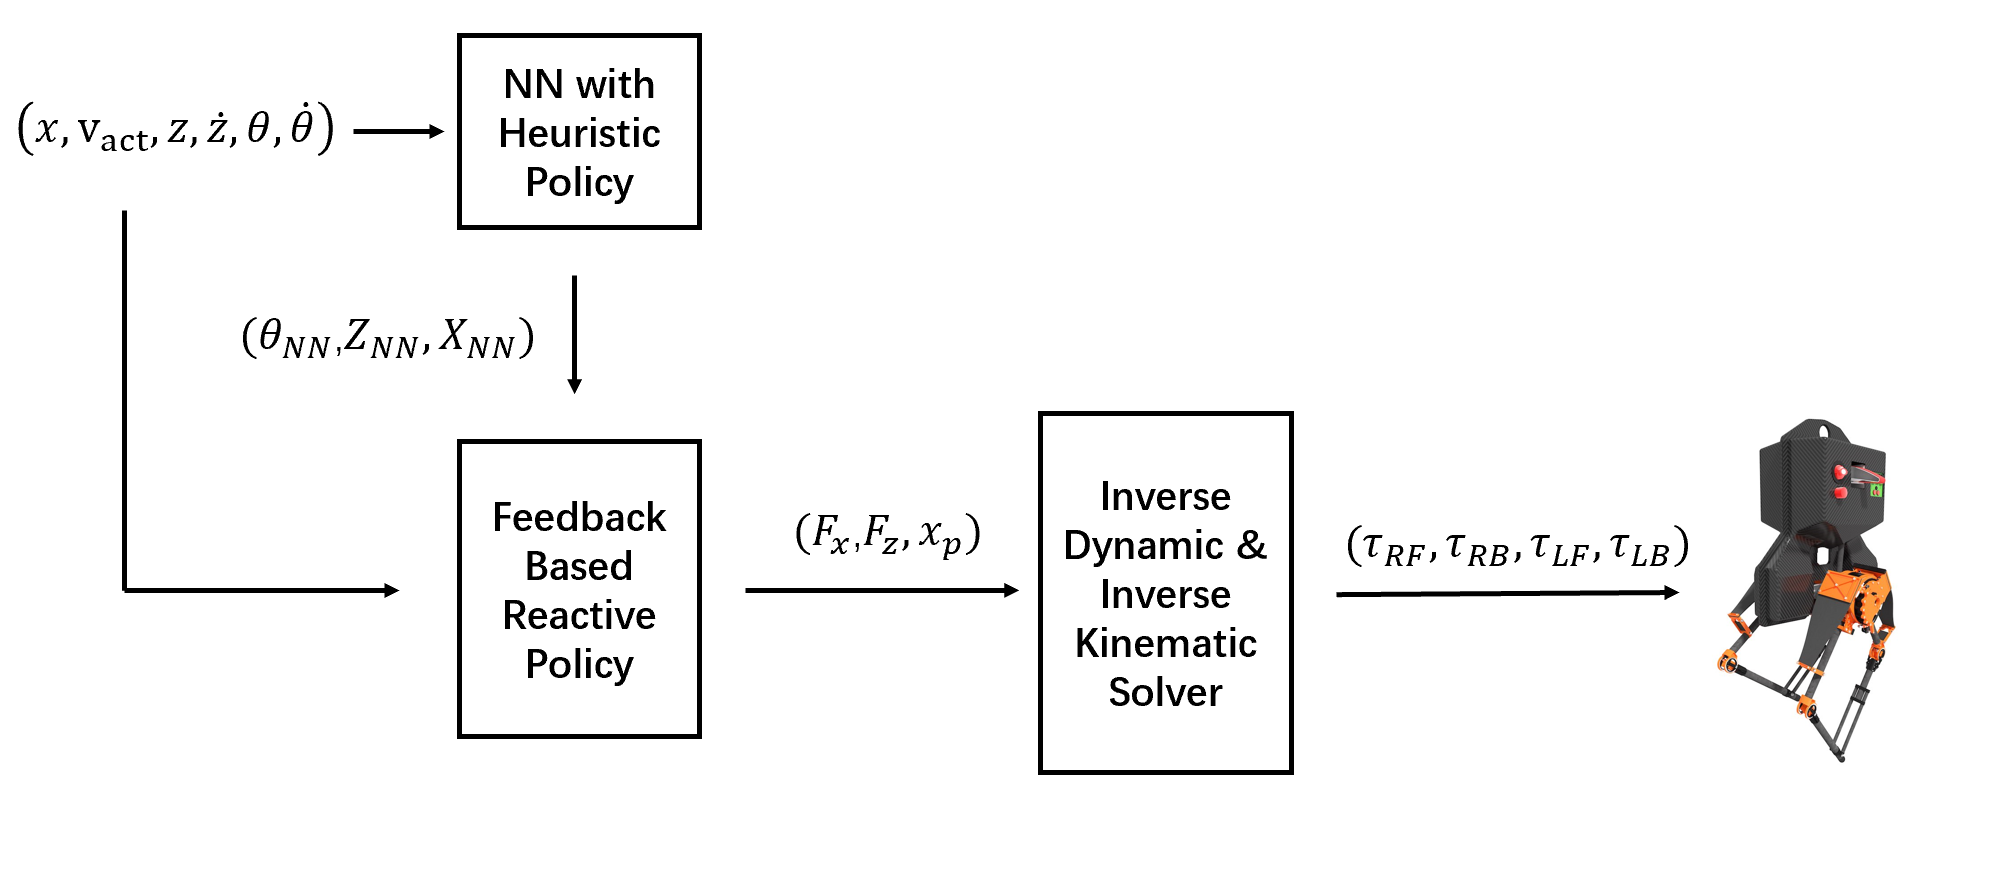
\includegraphics[width=.7\textwidth]{./img/Heuristic.PNG}
    \caption{Pipeline of our second neural network controller using a heuristic structure and neural network outputs for controlling ATRIAS. }
    \label{fig:H_process}
\end{figure}

There are several benefits to having such structure in our policies. First and foremost, the user can predict the behavior and understand the outputs of this policy. This is important for policies implemented on robots to ensure safety of the robot and its environment. 
%For example, controllers that use on inverse dynamics take torque constraints and other dynamics constraints into account. 
Moreover, if the user wants to test a slightly different setting than the simulation, she can easily tune other parameters of this policy, keeping the neural network fixed. Lastly, if the policy fails on hardware, it is easy for the user to understand why that might be, and even possible to fix other parts of the controller without re-training the neural network.


\section{Experiments with deep reinforcement learning}
In this section we describe our experiments with deep reinforcement learning for the ATRIAS bipedal robot. Our experiments compare a general neural network policy with a more structured policy, where the neural network helps modulate an expert controller. We compare both policies in simulation and hardware.

\subsection{Simulation Experiments}
%why doing simulation
We trained our neural network controllers in simulation before implementing on hardware. This is because we use Proximal Policy Optimization (PPO) as our learning algorithm. PPO needs to collect a large amount of data points at each iteration. When our current policy is not good enough, we would not be able to collect much data since the robot might fall at the very beginning of experiment. In order to collect enough number of data points, we need to do a large number of trials, making it near impossible to train on hardware. However, since we train our policies in simulation, the resulting controllers might work well in simulation environment but when implemented on hardware, they might fall. In order to overcome this issue, we add ground height disturbances to learn robust controllers in simulation. %Furthermore, while doing training, exploration can also be regarded as one kind of extra noise added to controllers.

\begin{figure}[t]
	\centering
	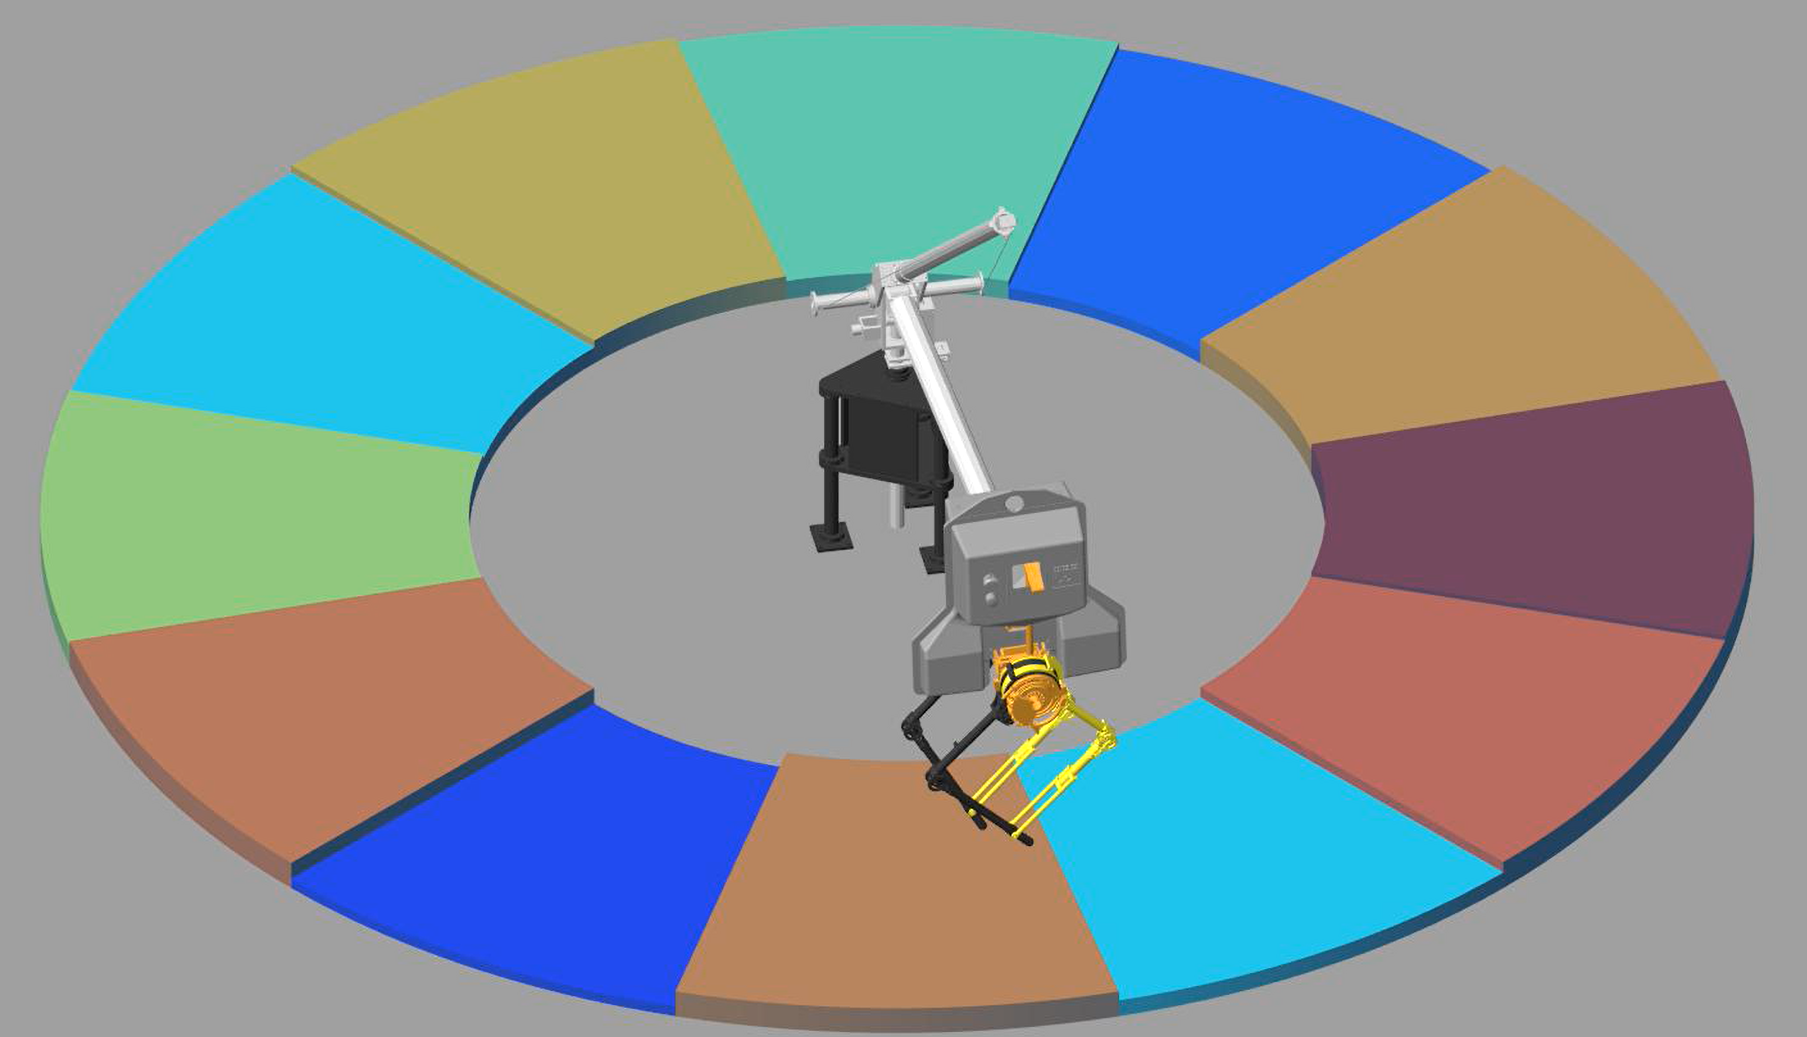
\includegraphics[width=.55\textwidth]{img/simulator.PNG}
    \caption{Simulation of ATRIAS with ground height disturbance. Different colors indicate different ground height disturbances. Maximum ground height disturbance is $\pm$ 10 cm. }
    \label{fig:process}
\end{figure}

The reward function is defined focusing on matching the desired walking speed and preventing large angular velocity of the torso. We also add a large penalty if the controller falls:
\begin{equation}
reward_t=\left\{
\begin{array}{rcl}
-C_1\cdot(v_{act, t}-v_{tgt})^2 -C_2\cdot(\dot{\theta}_t)^2 + 1 ,\  {if \ walk}\\
-C_3*T_{sim}, \  {if \ fall}
\end{array} \right.
\label{reward_1}
\end{equation}

where $v_{act, t}$ is the vector is the actual forward velocity of the robot at time $t$, $v_{tgt}$ is the target velocity, $\dot{\theta}_t$ is the angular velocity of torso pitch, $T_{sim}$ is the simulation time, $C_1,C_2,C_3$ are positive fixed parameters. This kind of cost function is similar to prior work on optimizing locomotion controllers, and it can easily distinguish points that walk from points that fall. The longer the controller can survive, the closer to the target speed, the less torso pitch the higher total reward the controller can get.
In this setting,$C_1 = 1$, $C_2=0.3$, $C_3=0.01$.
%One thing needs to be remarked is that the total reward does not directly indicate the robustness of the controller. For instance, a controller can overcome ground height disturbance might not have a high reward because it suffers from large penalty of large torso pitch which make the controller hard to be implemented on hardware. Anyway, the longer the controller can survive, the closer to the target speed, the less torso pitch the higher total reward the controller can get and more likely to work on hardware.
In our observation, often the highest scoring controllers in simulation tend to exploit simulation inaccuracies. For example, some controllers tend to jerk the torso to achieve speeds closer to the target speed. While these perform well in simulation, they tend to fail on hardware. 


%\TL{Explain the set up. How many data points per iteration? 3 runs of best controller? }%we also set our data collection number up to more than 3 full simulation episodes data, so if the controller fall in simulation, we would collect more episodes of data so that we can collect enough data in one iteration.

\subsubsection{Neural Network Policy}
The first set of simulation experiments were with the Neural Network Policy (NN Policy), described in Section \ref{NN_P}. The first step for Neural Network Policy was behavior cloning. After initialization, our NN policy could walk on flat ground, but it had difficulties with ground height disturbances. This was unsurprising because the 'expert controller' also cannot walk on ground with ground height disturbance. Hence, we had to train the policy further to achieve acceptable performance.
%More importantly, the 'expert controller' has a jump up behavior at the beginning of walking, and our initialization of NN policy also inherited this behavior. In simulation, this behavior would not lead to falling, but on hardware, ATRIAS would fall as soon as it tries to start walking because of the initial jump.

\begin{figure}[t]
	\centering
	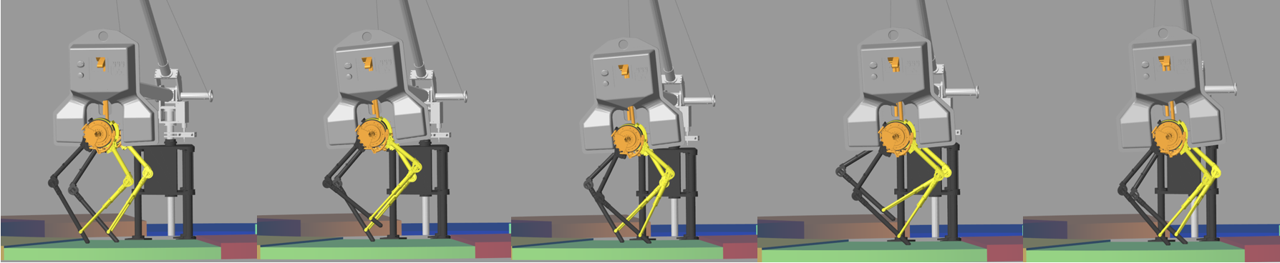
\includegraphics[width=.55\textwidth]{./img/NN_walking.png}
    \caption{Sequence of frames from a single walking cycle (left to right). }
    \label{fig:NN_walking}
\end{figure}

%After initialization, we used DRL to improve the performance of our policy. 
We trained 10 different NN policies, the rewards for which are shown on Figure \ref{fig:Reward}. The rewards shown is the averaged reward of one iteration which consisted on 30,000 data points. %To reduce the influence of luck,  
As shown in the plot, the reward keeps growing as training goes on, starting from the average cost of the expert. This shows that PPO achieves a very stable training with little to no forgetting of the initial expert.

\begin{figure}[t]
	\centering
	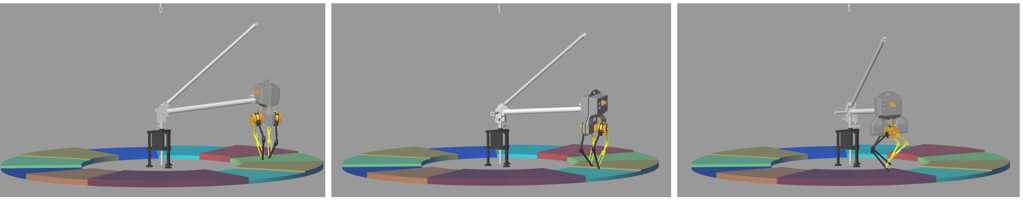
\includegraphics[width=.65\textwidth]{img/NN_walking_2.png}
    \caption{A time lapse of Neural Network Policy walking around the boom with ground height disturbance in simulation. }
    \label{fig:NN_walking_2}
\end{figure}

\begin{figure}[t]
	\centering
	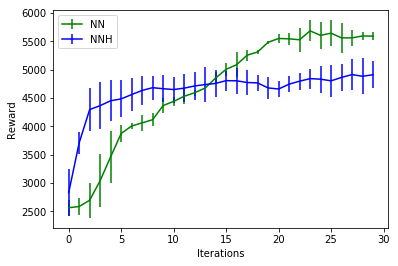
\includegraphics[width=.65\textwidth]{img/NN_H_reward.png}
    \caption{Training plot of Neural Network Policy (green) and Neural Network with Heuristic Policy (blue). Each of them is averaged of 5 trials data. In our training, we collected 30000 data in one iteration. For each simulation episode, we simulated 10 seconds if the controller keeps walking, and in simulation our time step was 0.001s. Thus, we could collect no more than 10000 data in a single episode, which also means in one iteration we needed data at least from 3 different episodes. By collecting data from more than one episodes, we could average the total rewards to determine the performance of the controller, also eliminating `lucky' runs.}
    \label{fig:Reward}
\end{figure}

\begin{figure}[t]
	\centering
	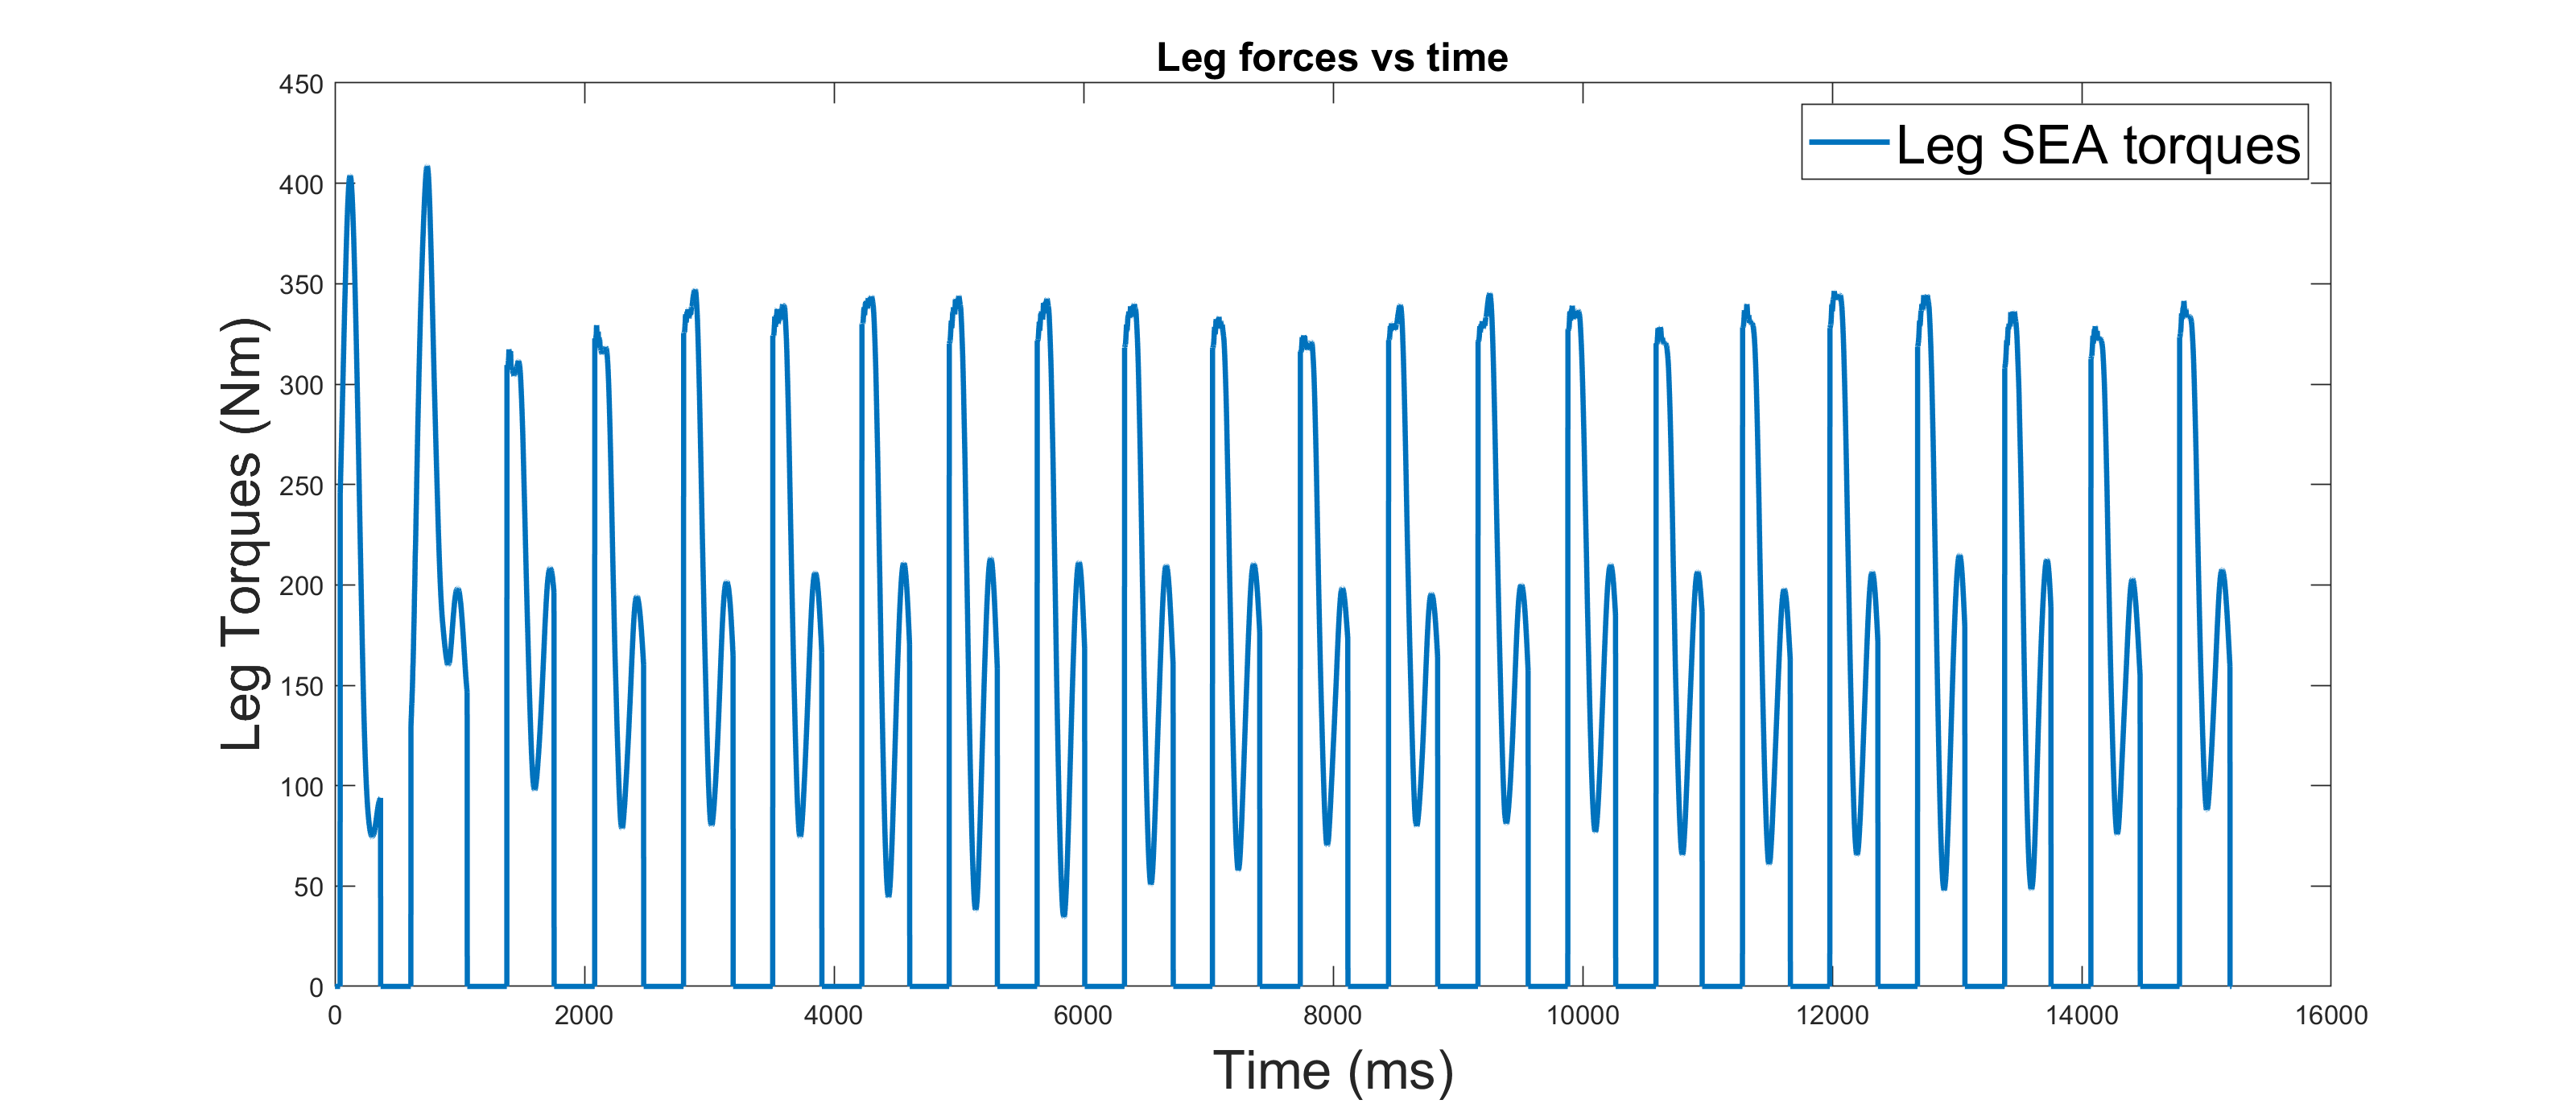
\includegraphics[width=.65\textwidth]{img/leg_force_profie.png}
    \caption{A plot of the stance leg SEA torques measured during one run of the NN policy on hardware. The torques are 0 during swing and follow a double hump pattern in stance. Note the high initial torques in the first two steps as compared to the rest of the walking cycle.}
    \label{fig:NN_walking_hw}
\end{figure}
The NN policy achieved good reward improvement compared to the initialization. After training, the NN policy could walk with ground height disturbance with a reasonable success rate. Figure \ref{fig:NN_walking} and Figure \ref{fig:NN_walking_2} shows the NN policy walking with ground height disturbance.


\subsubsection{Neural network with heuristic policy}

The second set of simulation experiment uses a neural network in a heuristic policy, described in section \ref{NN_HP}. %This heuristic policy don't have to do behavior cloning, we only initialized the outputs of Heuristic Policy to match the parameters of the 'expert controller'. 
By initializing this policy to the target values of the 'expert controller', the initial policy was able to walk on flat ground but cannot walk on rough ground. %And it still has a starting jump behavior.

The training plot of Heuristic Policy is shown on Figure \ref{fig:Reward}. As shown on the plot, the Heuristic Policy reward improves faster than the NN policy but reaches its peak in very few iterations. It then remains at that reward for the rest of iterations. The initial fast improvement is expected because as the heuristic policy uses the structure of the feedback-based reactive stepping policy, the search for reasonable parameters is simple. Hence, walking controllers are found much faster. However, the same structure also imposes a strong bias on the search, and as a result, it is hard to find controllers that can perform as well as the pure NN controller in simulation. However, as we describe later, even though the best reward achieved by Heuristic controllers is lower, the rate of transfer to hardware is much higher than the NN policy.

\begin{figure}[t]
	\centering
	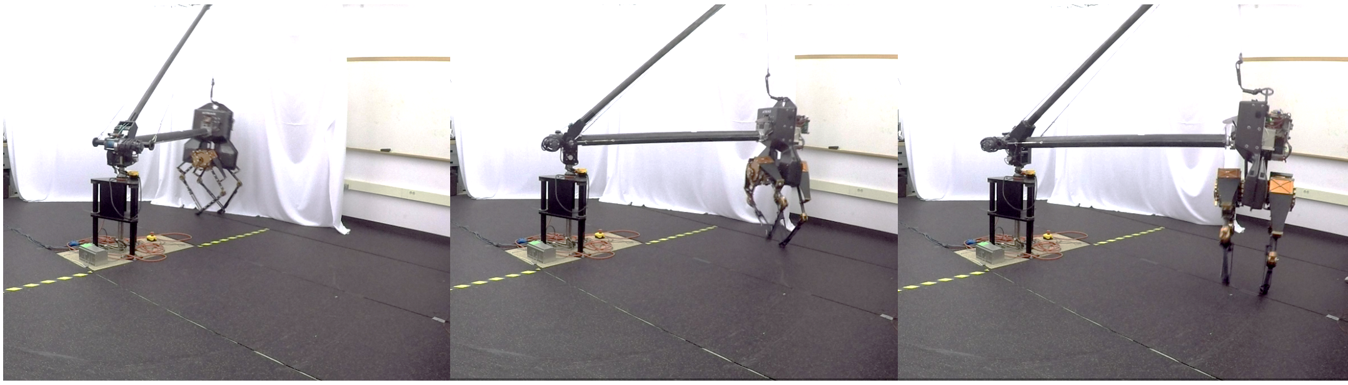
\includegraphics[width=.85\textwidth]{img/Hardware.PNG}
    \caption{A time lapse of ATRIAS walking around the boom during a run of a NN with heuristic policy.}
    \label{fig:Hardware_walking}
\end{figure}

\subsection{Hardware Experiments}
\label{sec:nn_expts}
We tested 5 NN policies and 5 heuristic policies in our first set of hardware experiment, with the reward function described in Function \ref{reward_1}. 

There is a large mismatch between simulation and hardware starting conditions for our system. Starting from rest is a significant challenge for bipedal robots, especially underactuated robots like ATRIAS. ATRIAS is incapable of balancing by standing in place, and needs to continue stepping to stay upright. Typically, a start-up routine is designed for these robots to reach some initial walking gait, and then the controller to be tested is initiated. For example \cite{hubicki2016atrias} start by executing a stepping motion in air, and a human holds on to the robot as its lowered onto the ground. We train our controllers to start from rest in both simulation and hardware, to avoid having to design a start-up routine. However, our simulation leg is not initially loaded, so the simulation has to make an initial push to keep the CoM from going too low. On the other hand, on hardware the robot starts in position control in the air and then is lowered. So as stance starts, there is already sufficient force in the leg, and the initial push (from simulation) makes the robot leave ground. Such a controller falls on hardware. This behavior is illustrated in Figure \ref{fig:NN_walking_hw} where the first two steps on hardware experience higher leg forces than the rest of the steps.

\subsubsection{Neural network policy}

2 out of 5 of the NN policy could walk on hardware. But all of the NN policies shared the same issue that at the beginning of walking they would jump up. This behavior can also be seen in our simulation. The initializing 'expert controller' has a jump up behavior at the beginning of walking, and our NN policy also inherits this behavior. In simulation, this behavior would not lead to falling, but on hardware, ATRIAS would fall as soon as it tries to start walking because of the initial jump. On hardware, 2 out of 5 controllers could overcome the initial disturbance and then started normal walking pattern. 3 out 5 controllers, however could not recover from this disturbance. This led to a \textbf{$40\%$} rate of transfer of learned policies between simulation and hardware.

\subsubsection{Neural network with heuristic policy}

4 out 5 controllers trained with neural network as part of the heuristic structure were able to walk on hardware. There are a few reasons for the success of the NN with heuristic structure policy, over the pure NN policy. Firstly, the initial discrepancy between simulation and hardware leg force is already compensated for by the heuristic structure. In the simulation, the NN predicts a desired height, and the feedback on this desired height results in a high leg force, as the actual height of the robot is lower. On hardware, the actual height of the robot is close to this desired height, so it automatically reduces the initial leg force. Unlike pure NN policy, where the forces were high on both simulation and hardware, now the initial forces are only high when the actual state of the robot is different from the desired. This structure in our policy, hence, makes the generalization from simulation to hardware very simple and intuitive.

Secondly, since the structure of the policy is readable by an expert, the expert can still edit the policy after being trained in simulation. For example, if the NN was trained on a lower velocity but the expert wanted to run the robot on a higher velocity, the heuristic structure allows to directly edit this target. Similarly, we observed that some of our controllers were falling because of speeding, and we increased the feedback gain $k$ on velocity feedback, described in Equation \ref{x_p eq}. This modification significantly improved the success rate of policies learned in simulation on hardware.

These experiments highlight the advantages of structure in learned policies. While the NN helped us improve our heuristic policy, as shown in Figure \ref{fig:Reward}, by learning a state-dependant desired height, pitch and footstep location, it also kept the intuitive structure of the heuristic. So, it was able to better reject disturbances between simulation and hardware, as well as be modified for slightly different test situations, without needing re-learning. This allowed a \textbf{$80\%$} rate of transfer of learned policies between simulation and hardware.
